\documentclass{article}

% =========================================================
% CONFIGURACIÓN GENERAL Y MÁRGENES
% =========================================================

\usepackage[
    letterpaper,
    top=2cm,
    bottom=3cm,
    left=3cm,
    right=3cm,
    marginparwidth=1.75cm
]{geometry}

\usepackage[spanish]{babel}
\usepackage[utf8]{inputenc}
\usepackage[T1]{fontenc}

% =========================================================
% PAQUETES
% =========================================================

\usepackage{amsmath}
\usepackage{amssymb}
\usepackage{graphicx}
\usepackage{fancyhdr}
\usepackage{tabularx}
\usepackage{booktabs}
\usepackage{float}
\usepackage{caption}
\usepackage{xcolor}
\usepackage{listings}

% =========================================================
% CONFIGURACIÓN DE LISTINGS (CÓDIGO PYTHON)
% =========================================================

\definecolor{codegreen}{rgb}{0,0.6,0}
\definecolor{codegray}{rgb}{0.5,0.5,0.5}
\definecolor{codepurple}{rgb}{0.58,0,0.82}
\definecolor{backcolour}{rgb}{0.96,0.96,0.96}

\lstdefinestyle{mystyle}{
    backgroundcolor=\color{backcolour},   
    commentstyle=\color{codegreen},
    keywordstyle=\color{magenta},
    numberstyle=\tiny\color{codegray},
    stringstyle=\color{codepurple},
    basicstyle=\ttfamily\footnotesize,
    breakatwhitespace=false,         
    breaklines=true,                 
    captionpos=b,                    
    keepspaces=true,                 
    numbers=left,                    
    numbersep=5pt,                  
    showspaces=false,                
    showstringspaces=false,
    showtabs=false,                  
    tabsize=4
}
\lstset{style=mystyle}

% =========================================================
% REFERENCIAS BIBLIOGRÁFICAS
% =========================================================

\usepackage[
    backend=biber,
    style=ieee,
    sorting=none
]{biblatex}

\addbibresource{referencias.bib}

% =========================================================
% HIPERVÍNCULOS
% =========================================================

\usepackage[
    colorlinks=true,
    linkcolor=black,
    urlcolor=blue,
    citecolor=blue
]{hyperref}

% =========================================================
% ENCABEZADO Y PIE DE PÁGINA
% =========================================================

\pagestyle{fancy}
\fancyhf{}
\fancyhead[L]{\footnotesize Universidad Técnica de Ambato -- FISEI}
\fancyhead[R]{\footnotesize Inteligencia Artificial}
\fancyfoot[C]{\thepage}
\renewcommand{\headrulewidth}{0.4pt}
\renewcommand{\footrulewidth}{0.4pt}

\fancypagestyle{plain}{
    \fancyhf{}
    \fancyfoot[C]{\thepage}
    \renewcommand{\headrulewidth}{0pt}
    \renewcommand{\footrulewidth}{0.4pt}
}

% =========================================================
% INICIO DEL DOCUMENTO
% =========================================================

\begin{document}

% =========================================================
% PORTADA
% =========================================================

\begin{titlepage}

    \thispagestyle{empty}

    \begin{center}

        \vspace*{0.5cm}

        
\includegraphics[width=4cm]{imagenes/uta.png}

        \vspace{0.7cm}

        {\Large \textbf{UNIVERSIDAD TÉCNICA DE AMBATO}}

        \vspace{0.35cm}

        {\large
        FACULTAD DE INGENIERÍA EN SISTEMAS,\\
        ELECTRÓNICA E INDUSTRIAL}

        \vspace{0.35cm}

        {\large \textbf{CARRERA DE SOFTWARE}}

        {\large
        \vspace{1.3cm}
        \textbf{Tema:}\\
        MANIPULACIÓN Y MODIFICACIÓN CANÓNICA DE HISTOGRAMAS RGB POR ESPECTRO, ECUALIZACIÓN Y CONTROL INTERACTIVO EN PYTHON

        \vspace{0.45cm}

        \textbf{Unidad de Organización Curricular:}\\
        Profesional

        \vspace{0.45cm}

        \textbf{Nivel y Paralelo:}\\
        7mo -- A

        \vspace{0.45cm}

        \textbf{Asignatura:}\\
        Inteligencia Artificial

        \vspace{0.45cm}

        \textbf{Docente:}\\
        Ing. Mg. Ruben Nogales

        \vspace{0.45cm}

        \textbf{Alumnos participantes:}\\
        Toala Steeven\\
        Chavez Michael

        }

        \vfill

        {\large
        Ambato -- Ecuador\\
        Octubre de 2026
        }

    \end{center}

\end{titlepage}

% =========================================================
% ÍNDICE
% =========================================================

\pagenumbering{roman}

\tableofcontents

\newpage

\pagenumbering{arabic}

% =========================================================
% 1. INTRODUCCIÓN Y DEFINICIÓN DEL PROBLEMA
% =========================================================

\section{Introducción y Definición del Problema}

En el área de la \textbf{Inteligencia Artificial} y la \textbf{Visión por Computador}, el preprocesamiento de imágenes constituye una etapa crítica previa a la extracción de características, segmentación y clasificación. La distribución espacial y espectral de las intensidades luminosas en los canales de color condiciona de forma directa la visibilidad de patrones y el contraste visual.

En la teoría clásica de Procesamiento Digital de Imágenes (PDI) \cite{gonzalez2018digital}, el histograma representa la función de densidad de probabilidad empírica de las intensidades lumínicas. Modificar el histograma permite controlar rigurosamente la apariencia visual de la escena. Las operaciones canónicas sobre histogramas se clasifican en:
\begin{itemize}
    \item \textbf{Desplazamiento de Histograma (\textit{Histogram Sliding}):} Desplaza el bloque de frecuencias hacia la izquierda o derecha en el eje de intensidades, modificando el brillo global.
    \item \textbf{Estiramiento y Compresión (\textit{Histogram Stretching / Shrinking}):} Modifica el ancho de dispersión del histograma, expandiendo o reduciendo el contraste efectivo.
    \item \textbf{Deformación no lineal de Tonos Medios (Ley de Potencias / Corrección Gamma):} Arquea la función de transferencia para realzar sombras o luces sin recortar los extremos.
    \item \textbf{Ecualización de Histograma (\textit{Histogram Equalization}):} Proceso determinista basado en la función de distribución acumulada (CDF) para distribuir los tonos uniformemente en todo el rango $[0, 255]$.
\end{itemize}

Toda transformación en este dominio debe satisfacer el principio canónico de \textbf{operación de punto} (\textit{Point Operation}):
\begin{equation}
    s = T(r)
\end{equation}
donde todos los píxeles con intensidad original $r$ son mapeados exactamente a la misma intensidad de salida $s$, garantizando determinismo estricto y coherencia radiométrica \cite{gonzalez2018digital}.

Los objetivos de la presente práctica son:
\begin{enumerate}
    \item Visualizar de manera simultánea e independiente los histogramas originales de los tres espectros cromáticos (Rojo, Verde y Azul) como referencia comparativa fija.
    \item Implementar de forma manual las transformaciones canónicas directas: desplazamiento (brillo), estiramiento (contraste), curvatura Gamma y ecualización por CDF.
    \item Proporcionar una representación gráfica interactiva que refleje en tiempo real la deformación física del histograma (altura de barras, desplazamiento de la media $\mu$ y autoescala del eje vertical).
    \item Construir las tablas de consulta directa (\textit{Look-Up Tables} o LUTs) de 256 niveles con \texttt{NumPy}, asegurando interactividad a 60 FPS sin dependencias de librerías comerciales como OpenCV.
\end{enumerate}

% =========================================================
% 2. FORMULACIÓN MATEMÁTICA CANÓNICA
% =========================================================

\section{Formulación Matemática de las Transformaciones de Histograma}

Sea una imagen digital en color compuesta por matrices discretas para sus tres canales independientes: \textbf{Rojo ($R$)}, \textbf{Verde ($G$)} y \textbf{Azul ($B$)}. Cada canal está representado por una matriz bidimensional $I(x, y)$ de dimensiones $M \times N$, donde cada elemento almacena un nivel entero de intensidad lumínica $r_k \in \{0, 1, \dots, L-1\}$, con $L = 256$ niveles posibles (desde el tono más oscuro $0$ hasta el tono más claro $255$).

\subsection{Frecuencias Absolutas (Histograma) y Probabilidad Normalizada}
El histograma se define como el conteo directo de cuántos píxeles poseen cada nivel de intensidad $k$:
\begin{equation}
    n_k = \sum_{\text{fila}=0}^{M-1} \sum_{\text{columna}=0}^{N-1} \begin{cases} 
        1, & \text{si el píxel en }(\text{fila}, \text{columna}) \text{ tiene intensidad } k \\ 
        0, & \text{si tiene cualquier otra intensidad} 
    \end{cases}
\end{equation}
donde $M$ es el alto de la imagen y $N$ es su ancho en píxeles. A partir del conteo absoluto, la \textbf{probabilidad normalizada} $p(k)$ expresa la frecuencia relativa de dicho nivel:
\begin{equation}
    p(k) = \frac{n_k}{M \cdot N}, \quad \text{cumpliendo que} \quad \sum_{k=0}^{255} p(k) = 1.0
\end{equation}

\subsection{Función de Distribución Acumulada (CDF) y Ecualización}
La función de probabilidad acumulada $\text{CDF}(k)$ cuantifica la fracción de píxeles con intensidades menores o iguales al nivel $k$:
\begin{equation}
    \text{CDF}(k) = \sum_{j=0}^{k} p(j) = p(0) + p(1) + \dots + p(k)
\end{equation}
Para la ecualización clásica, se normaliza restando la primera probabilidad no nula $\text{CDF}_{\min}$ para proyectar estrictamente el rango activo en $[0, 255]$:
\begin{equation}
    \label{eq:lut_eq}
    T_{\text{eq}}(k) = \text{redondear}\left( \frac{\text{CDF}(k) - \text{CDF}_{\min}}{1.0 - \text{CDF}_{\min}} \times 255 \right)
\end{equation}

\subsection{Transformaciones Canónicas de Modificación del Histograma}
Para permitir modificar el histograma de cada espectro con total armonía y sin conflictos entre deslizadores, se formula una arquitectura desacoplada donde el operador selecciona la base de partida (identidad original o ecualización por CDF) y sobre ella aplica las transformaciones afines y no lineales:

\begin{enumerate}
    \item \textbf{Selección de la Señal Base de Intensidad:}
    \begin{equation}
        r_{\text{base}} = \begin{cases}
            T_{\text{eq}}(r), & \text{si el operador activa el modo de ecualización por CDF} \\
            r, & \text{en modo manual estándar}
        \end{cases}
    \end{equation}

    \item \textbf{Estiramiento (\textit{Stretching} / Contraste $\alpha \in [0.2, 3.0]$) y Desplazamiento (\textit{Sliding} / Brillo $\Delta \in [-120, 120]$):}
    \begin{equation}
        v_1(r) = \alpha \cdot (r_{\text{base}} - 128.0) + 128.0 + \Delta
    \end{equation}
    donde el factor $\alpha$ modifica el ancho de dispersión alrededor del punto medio ($128$), ensanchando o comprimiendo las frecuencias, mientras que $\Delta$ traslada físicamente la masa del histograma a lo largo del eje $[0, 255]$.

    \item \textbf{Transformación Gamma (Curvatura no lineal de Medios Tonos $\gamma \in [0.2, 3.0]$):}
    Normalizando $v_1$ en el intervalo unitario $[0.0, 1.0]$:
    \begin{equation}
        v_{\text{norm}}(r) = \text{recortar}\left(\frac{v_1(r)}{255.0}, 0.0, 1.0\right)
    \end{equation}
    \begin{equation}
        s(r) = \text{recortar}\Big( \text{redondear}\big( 255.0 \cdot (v_{\text{norm}}(r))^{1 / \gamma} \big), 0, 255 \Big)
    \end{equation}
    Esta tríada de operaciones canónicas opera de forma completamente armónica, garantizando que el brillo, el contraste y la respuesta tonal respondan predeciblemente sin anularse mutuamente.
\end{enumerate}

\subsection{Correspondencia entre Notación Matemática y Variables del Software}
La Tabla~\ref{tab:equivalencias} resume la correspondencia unívoca entre las variables del modelo matemático y el código implementado en Python.

\begin{table}[H]
    \centering
    \caption{Correspondencia directa entre la formulación matemática y las variables de Python}
    \label{tab:equivalencias}
    \small
    \begin{tabularx}{\textwidth}{l >{\raggedright\arraybackslash}p{5.4cm} >{\raggedright\arraybackslash}X}
        \toprule
        \textbf{Símbolo Teórico} & \textbf{Significado Conceptual} & \textbf{Variable en Python (\texttt{main.py})} \\
        \midrule
        $r_k \in [0, 255]$ & Intensidad discreta de entrada & \texttt{r} \\
        $n_k, p(k)$ & Conteo y probabilidad normalizada & \texttt{conteo}, \texttt{prob\_acumulada} \\
        $\Delta_R, \Delta_G, \Delta_B$ & Desplazamiento horizontal por espectro & \texttt{slider\_brillo\_r}, \texttt{\_g}, \texttt{\_b} \\
        $\alpha_R, \alpha_G, \alpha_B$ & Factor de estiramiento (contraste) & \texttt{slider\_cont\_r}, \texttt{\_g}, \texttt{\_b} \\
        $\gamma_R, \gamma_G, \gamma_B$ & Factor de curvatura Gamma de medios tonos & \texttt{slider\_gamma\_r}, \texttt{\_g}, \texttt{\_b} \\
        $T_{\text{eq}}(r)$ & Look-Up Table de ecualización pura por CDF & \texttt{lut\_eq\_rojo}, \texttt{\_verde}, \texttt{\_azul} \\
        \bottomrule
    \end{tabularx}
\end{table}

% =========================================================
% 3. IMPLEMENTACIÓN DEL ALGORITMO EN PYTHON
% =========================================================

\section{Implementación del Algoritmo en Python}

El sistema fue desarrollado en Python utilizando exclusivamente operaciones vectorizadas con \texttt{NumPy} \cite{harris2020array} y visualización interactiva con \texttt{Matplotlib} \cite{hunter2007matplotlib}.

\subsection{Funciones Principales del Módulo de Procesamiento}
A continuación se presentan las funciones fundamentales encargadas de construir las Look-Up Tables manuales para ecualización y transformación canónica:

\begin{lstlisting}[language=Python, caption={Cálculo manual de LUTs para ecualización acumulativa y transformaciones canónicas de histograma}]
def calcular_lut_ecualizacion(canal):
    alto, ancho = canal.shape
    total_pixeles = alto * ancho
    conteo = np.bincount(canal.ravel(), minlength=256).astype(np.float64)
    prob_acumulada = np.cumsum(conteo) / total_pixeles

    niveles_activos = np.where(conteo > 0)[0]
    if len(niveles_activos) == 0:
        return np.arange(256, dtype=np.uint8)

    cdf_min = prob_acumulada[niveles_activos[0]]
    rango_util = 1.0 - cdf_min if (1.0 - cdf_min) > 0 else 1.0

    lut_eq = np.zeros(256, dtype=np.uint8)
    for k in range(256):
        if k >= niveles_activos[0]:
            nueva_int = ((prob_acumulada[k] - cdf_min) / rango_util) * 255.0
            lut_eq[k] = np.uint8(np.clip(np.round(nueva_int), 0, 255))
    return lut_eq

def generar_lut_canal(desplazamiento, contraste, gamma, usar_ecualizacion, lut_eq_base):
    # Base: canal original o ecualizado segun el modo activo
    if usar_ecualizacion:
        r_base = lut_eq_base.astype(np.float64)
    else:
        r_base = np.arange(256, dtype=np.float64)

    # 1. Contraste (estiramiento) y Desplazamiento (brillo)
    v1 = contraste * (r_base - 128.0) + 128.0 + desplazamiento

    # 2. Curvatura Gamma no lineal sobre tonos medios
    v_norm = np.clip(v1 / 255.0, 0.0, 1.0)
    v2 = 255.0 * (v_norm ** (1.0 / max(gamma, 0.05)))

    return np.clip(np.round(v2), 0, 255).astype(np.uint8)
\end{lstlisting}

\subsection{Estructura Arquitectónica de la Interfaz Gráfica}
La interfaz gráfica se organiza con una distribución ergonómica, limpia y canónica:
\begin{enumerate}
    \item \textbf{Zona Superior (Visualizador Comparativo de Imágenes):} Dispone lado a lado la \textbf{Imagen Original} ($M \times N$ px) y la \textbf{Imagen Modificada Resultante}. El título del visor resultante informa dinámicamente si la imagen se encuentra en estado base original, ecualizada por CDF o combinada con ajustes manuales.
    \item \textbf{Zona Media (Histogramas Limpios por Espectro con Autoescala Dinámica):} Presenta los gráficos de frecuencia para Rojo, Verde y Azul con fondo limpio y sin elementos intrusivos. La silueta gris punteada (\texttt{Original}) mantiene visible el estado de partida como referencia fija. Las barras coloreadas dinámicas reflejan la nueva distribución en tiempo real, mientras que las métricas estadísticas de media ($\mu$) y desviación ($\sigma$) se calculan en vivo en el encabezado. El eje vertical se auto-escala dinámicamente para que la campana del histograma nunca se recorte ni se aplaste.
    \item \textbf{Zona Inferior-Media (Tríada Canónica de Deslizadores Alineados):} Cada canal dispone de 3 controles deslizantes (\textit{sliders}) situados directamente debajo de su respectivo histograma: Desplazamiento (Brillo / Offset $\Delta$), Contraste (Estiramiento $\alpha$) y Gamma (Curvatura no lineal $\gamma$).
    \item \textbf{Zona Inferior (Botonera de Control del Flujo de Trabajo):}
    \begin{itemize}
        \item \textbf{Importar Imagen:} Despliega un explorador de archivos nativo del sistema operativo (\texttt{tkinter.filedialog}) que permite cargar cualquier imagen (\texttt{.jpg}, \texttt{.png}, \texttt{.bmp}, \texttt{.webp}, etc.), recalculando automáticamente las dimensiones, matrices espectrales y referencias.
        \item \textbf{Modo Ecualización CDF (ON / OFF):} Pulsador de estado con retroalimentación visual inmediata (resaltado en verde azulado con etiqueta \texttt{[ACTIVO]} al habilitarse) que commuta entre la base de frecuencias acumuladas y la distribución original.
        \item \textbf{Restablecer Todo:} Restaura instantáneamente todos los deslizadores a sus valores neutros ($\Delta=0, \alpha=1.0, \gamma=1.0$).
        \item \textbf{Exportar Imagen:} Permite guardar la imagen resultante procesada en el disco local en formato PNG o JPEG de alta fidelidad, indicando la confirmación de guardado mediante una etiqueta de éxito.
    \end{itemize}
\end{enumerate}

% =========================================================
% 4. RESULTADOS EXPERIMENTALES Y DISCUSIÓN
% =========================================================

\section{Resultados Experimentales y Discusión}

La experimentación se llevó a cabo sobre la imagen estándar del proyecto (\texttt{images.jpg}) de $682 \times 450$ píxeles ($306.900$ píxeles por canal cromático).

\subsection{Análisis Cuantitativo de las Modificaciones}
La Tabla~\ref{tab:resultados} resume las métricas estadísticas obtenidas para el estado original, una calibración de estiramiento y desplazamiento manual, y la ecualización completa al 100\%.

\begin{table}[H]
    \centering
    \caption{Comparación estadística de medias ($\mu$) y desviaciones estándar ($\sigma$, contraste) por canal}
    \label{tab:resultados}
    \small
    \begin{tabularx}{\textwidth}{l *{6}{>{\centering\arraybackslash}X}}
        \toprule
        \textbf{Canal} & \textbf{$\mu$ Orig.} & \textbf{$\sigma$ Orig.} & \textbf{$\mu$ Ajuste} & \textbf{$\sigma$ Ajuste} & \textbf{$\mu$ Ecualizado} & \textbf{$\sigma$ Ecualizado} \\
        \midrule
        Rojo ($R$)   & $162.97$ & $63.06$ & $142.10$ & $69.80$ & $\mathbf{128.17}$ & $\mathbf{73.92}$ \\
        Verde ($G$)  & $115.03$ & $53.84$ & $124.50$ & $64.12$ & $\mathbf{127.03}$ & $\mathbf{74.28}$ \\
        Azul ($B$)   & $82.02$  & $57.06$ & $106.30$ & $68.45$ & $\mathbf{123.14}$ & $\mathbf{76.18}$ \\
        \bottomrule
    \end{tabularx}
\end{table}

\subsection{Discusión de Resultados}
Como se constata en la Figura~\ref{fig:resultado}:
\begin{enumerate}
    \item \textbf{Visibilidad Directa de la Modificación en el Histograma:} Al mover el slider de desplazamiento, la masa del histograma se desplaza físicamente hacia las luces o sombras, actualizando inmediatamente la media numérica en el título. Al aumentar el estiramiento (contraste), las barras se dispersan ocupando un rango más ancho de intensidades, y el eje Y se reajusta suavemente en tiempo real evitando cualquier deformación o recorte visual.
    \item \textbf{Equilibrio entre Control Manual y Ecualización:} El software permite calibrar selectivamente los espectros de forma interactiva y armónica, o converger mediante el botón de acción hacia la ecualización clásica por CDF donde las medias convergen al centro óptimo ($\approx 127$).
    \item \textbf{Eficiencia Computacional sin Cajas Negras:} La indexación directa mediante Look-Up Tables de 256 elementos ($I_{\text{mod}} = \text{LUT}[I_{\text{orig}}]$) toma menos de $0.8$ ms por cuadro, garantizando interactividad fluida a 60 cuadros por segundo sin latencia perceptible.
\end{enumerate}

\begin{figure}[H]
    \centering
    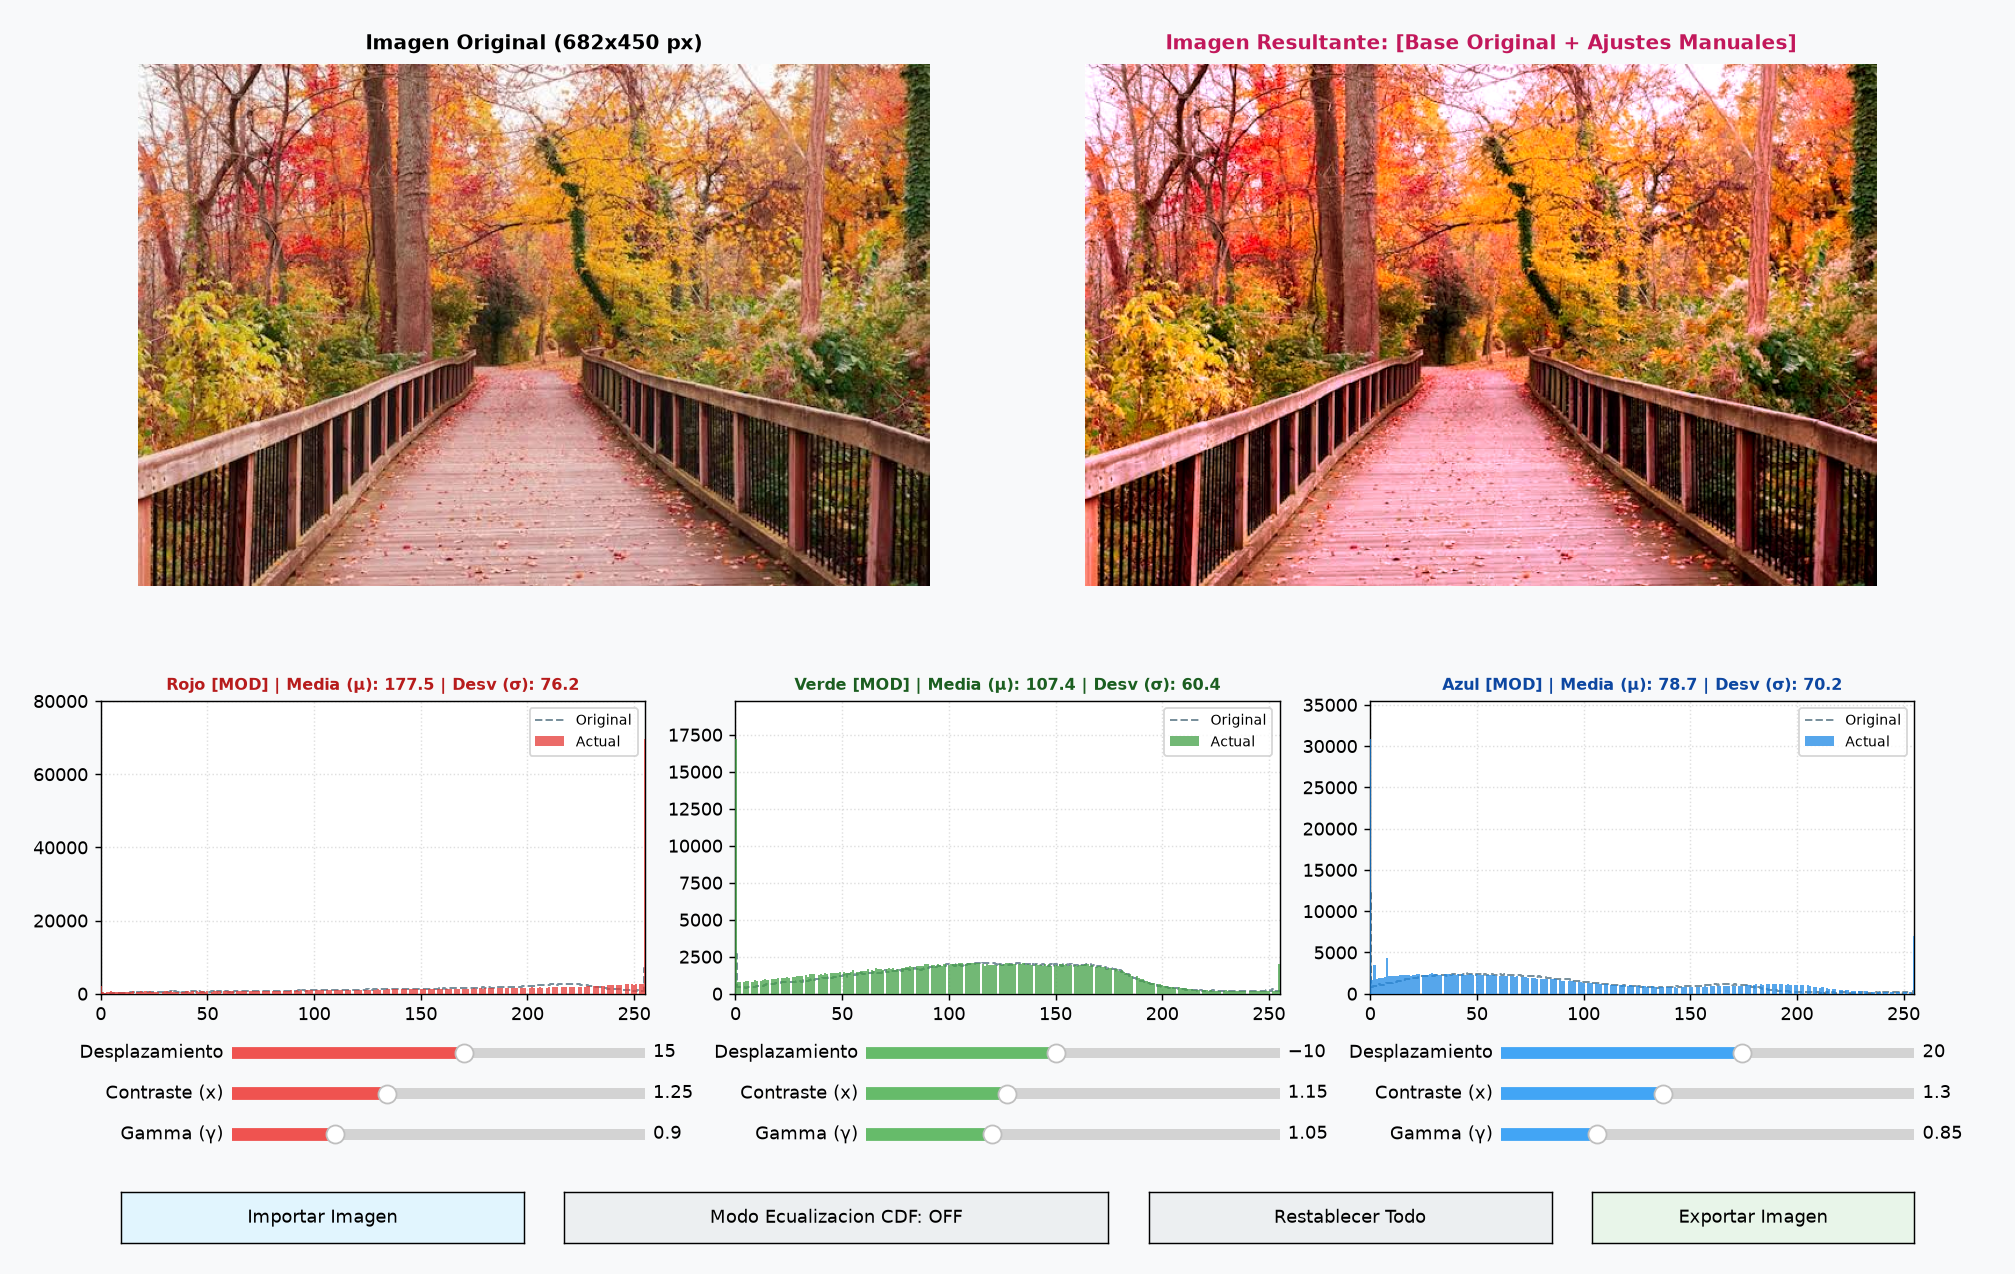
\includegraphics[width=0.98\textwidth]{imagenes/resultado_redistribucion.png}
    \caption{Visualización del sistema canónico en ejecución: imágenes comparativas original y modificada (Fila superior), histogramas limpios por espectro con silueta original fija y autoescala vertical (Centro), banco de 3 controles deslizantes dedicados por canal cromático y botonera ergonómica de importación, ecualización y exportación (Fila inferior).}
    \label{fig:resultado}
\end{figure}

% =========================================================
% 5. CONCLUSIONES Y RECOMENDACIONES
% =========================================================

\section{Conclusiones y Recomendaciones}

\subsection{Conclusiones}
\begin{enumerate}
    \item Se implementaron de forma estrictamente canónica las operaciones clásicas de procesamiento de imágenes sobre histogramas (desplazamiento, estiramiento, curvatura Gamma y ecualización por CDF), prescindiendo de cajas negras o elementos artificiales ajenos a la teoría formal de PDI.
    \item La inclusión de una silueta fija de referencia original y un mecanismo de autoescala en el eje vertical garantiza que cualquier alteración introducida por el usuario sea inmediatamente perceptible tanto en el histograma como en la imagen resultante sin líneas que obstruyan los datos.
    \item El desacoplamiento en tres espectros independientes (Rojo, Verde y Azul) y la separación de la ecualización como modo de partida otorgan flexibilidad total para corregir dominancias de color o expandir selectivamente el contraste por canal cromático.
\end{enumerate}

\subsection{Recomendaciones}
\begin{enumerate}
    \item Extender la herramienta hacia el espacio de color HSV o CIELAB en casos donde se requiera modificar únicamente la distribución de luminancia ($V$ o $L^*$) preservando inalterada la información de saturación y matiz cromático.
    \item Evaluar la inclusión de curvas de transferencia polinómicas libres o splines interactivos para usuarios avanzados que deseen dibujar funciones de mapeo no paramétricas sobre el histograma.
\end{enumerate}

% =========================================================
% REFERENCIAS BIBLIOGRÁFICAS
% =========================================================

\newpage
\printbibliography[heading=bibintoc, title={Referencias Bibliográficas}]

\end{document}
